\section*{Lezione 15}
\addcontentsline{toc}{section}{Lezione 15}

Le funzioni di cifratura e di decifratura che definiscono un crittosistema devono godere di diverse proprietà:

\begin{itemize}
	\item $\forall m \, \forall k \, D_k(E_k(m)) = m$
	In altre parole la funzione di cifratura e di decifratura sono una l'opposta dell'altra
	\item $\forall m \, \forall k$, la computazione di $c = E_k(m)$ e $D_k(c) = m$ dev'essere \textit{facile} (per Alice e Bob dev'essere facile decifrare, cifrare).
	\item Dev'essere \textit{estremamente difficile} trovare $c = E_k(m)$ senza conoscere $k$.
\end{itemize}

P.s.\textit{facile} è un problema risolvibile da una MDTD in tempo polinomiale, \textit{difficile} non è risolvibile in tempo polinomiale (non si conosce un algoritmo) (NP).

\subsection*{Cifrari storici}
\addcontentsline{toc}{subsection}{Cifrari storici}

\subsubsection*{Cifrario di Cesare}

Il primo cifrario storico conosciuto è quello di Cesare (scritto da Polibio forse). \'E un crittosistema simmetrico, quindi la chiave per cifrare/decifrare è la stessa; o meglio, la chiave per decifrare può essere ricavata \textit{facilmente} a partire dalla chiave per cifrare (e viceversa).

Nel cifrario di Cesare $PT = CT = \Sigma$ dove $\Sigma = \{A, B, C, ..., Z\}$, mentre $K = \{0, 1, 2, ..., 25\}$. Ogni lettera è cifrata indipendentemente dalle altre.

Come funziona? 
\begin{itemize}
	\item \textbf{Cifratura}: data una $k \in K$, per cirfrare una lettera del plaintext $\sigma$ si computa la funzione $E_k(\sigma)$ avanzando di $k$ posizioni lungo l'alfabeto, pertendo da $\sigma$ e riprendendo da A quando si raggiunge la Z
	\item \textbf{Decifratura}: data una chiave $k \in K$ e una lettera $c$ del ciphertext, si va indietro di $k$ posizioni lungo l'alfabeto (il contrario del precedente).
\end{itemize}

Esempi:
\begin{itemize}
	\item $E_3($\texttt{TRYAGAIN}$)=$ \texttt{WUBDJDLQ}
	\item $E_{25}($\texttt{IBM}$)=$ \texttt{HAL}
\end{itemize}

Esso è un crittosistema per sostituzione monoalfabetica: ogni lettera del testo in chiaro viene sostituita sempre con la stessa lettera nel testo cifrato (per una data $k$), ad esempio con $k=2$ la \texttt{a} diventa sempre una \texttt{c}.

Crittoanalisi: lo spazio delle chiavi è troppo piccolo (solo 25 chiavi possibili)! Quindi un attacco di forza bruta è possibile.


Alcune proprietà del cifrario di Cesare:
\begin{itemize}
	\item Commutatività: $E_3D_7E_6D_{11} = E_3E_6D_7D_{11} = E_{17} = D_9$
	\item Per tutte le $k \in \{1, 2, ..., 25\}$ vale la seguente proprietà:
	\begin{itemize}
		\item $D_k=E_{26-k}$
		\item $E_k=D_{26-k}$
		\item $D_kE_k=E_0=D_0$
	\end{itemize}
\end{itemize}

\subsubsection*{Cifrario di Hill}
Questo crittosistema si basa su algebra lineare. Associa alle lettere da A a Z dei numeri da 0 a 25, tutte le operazioni aritmetiche sono quindi effettuate $mod 26$.
Come funziona? Si sceglie un intero $d \geq 2$ (nell'esempio si utilizza proprio 2). La chiave di cifratura sarà una matrice quadrata $M$ di ordine $d$, invertibile in $\mathbb{Z}_{26}$ (ovvero deve esistere la matrice $M^{-1}$ dove i conti vengono fatti in resto 26). Per controllare che una matrice sia invertibile in $\mathbb{Z}_{26}$ si controlla che $det(M) \neq 0$.\\ 
La chiave di decifratura infatti è $M^{-1}$. 


Diciamo che $PT=CT=\Sigma^d$ dove $\Sigma=\{0, 1, 2,..., 25\}$.
\begin{itemize}
	\item \textbf{Cifratura}: il plaintext $m$ è diviso in blocchi di $d$ lettere ($m=P_1P_2...P_k$ con $|P_i|=d \; \forall i=1,2,...,l$).
	Se la lunghezza di $m$ non è multipla di $d$, si aggiungono dei caratteri \textit{dummy} (fittizie).\\
	Ogni blocco successivamente è cifrato separatamente: $C_i=M \cdot P_i \; \forall i = 1,2,...,l$. Il ciphertext è la concatenazione dei diversi blocchi $C_1, C_2, ..., C_l$.
	
	Esempio:
	$m =$ \texttt{HELP},
	\begin{equation*}
	M = \begin{bmatrix}
	3 & 3\\
	2 & 5
	\end{bmatrix}
	\end{equation*}
	
	\begin{equation*}
	M^{-1} = \begin{bmatrix}
    15 & 17\\
	20 & 9
	\end{bmatrix}
	\end{equation*}
	
	Abbiamo quindi:

	\[
	P_1 = \begin{bmatrix}
	H\\
	E
	\end{bmatrix}
	=
	\begin{bmatrix}
	7\\
	4
	\end{bmatrix}
	\;\;\;\;\;\;\;\;\;
	P_2 = \begin{bmatrix}
	L\\
	P
	\end{bmatrix}
	=
	\begin{bmatrix}
	11\\
	15
	\end{bmatrix}
	\]	
	
	\[
	C_1= M \cdot P_1 = \begin{bmatrix}
	3 & 3\\
	2 & 5
	\end{bmatrix} 
	\cdot \begin{bmatrix}
	7 \\
	4
	\end{bmatrix}
	=
	\begin{bmatrix}
	7\\
	8
	\end{bmatrix}
		=
	\begin{bmatrix}
	H\\
	I
	\end{bmatrix}
	\]
	
	\[
	C_2= M \cdot P_2 = \begin{bmatrix}
	3 & 3\\
	2 & 5
	\end{bmatrix} 
	\cdot \begin{bmatrix}
	11 \\
	15
	\end{bmatrix}
	=
	\begin{bmatrix}
	0\\
	19
	\end{bmatrix}
	=
	\begin{bmatrix}
	A\\
	T
	\end{bmatrix}
	\]
	
	Quindi, $c=C_1C_2$ = \texttt{HIAT}
	
	\item \textbf{Rompere il sistema:} Mettiamo che Eve scopre che $d=2$, ma non conosce $M$.
	A un certo punto vede che il testo cifrato $c=$ \texttt{HIAT} e dopo un po' scopre che quel messaggio voleva dire \texttt{HELP}.\\
	A questo punto sa che $HI = [7\; 8] = [H\; E] \cdot M = [7 \; 4] \cdot M$ e che\\
	$AT = [0\; 19] = [L\; P] \cdot M = [11 \; 15] \cdot M$. Da qui:
	\[
	M \cdot \begin{bmatrix}
	7 & 11\\
	4 & 15
	\end{bmatrix} 
	= \begin{bmatrix}
	7 & 0\\
	8 & 19
	\end{bmatrix}
	\]
	E da qui scopre che:
	\[
	M = \begin{bmatrix}
	7 & 0\\
	8 & 19
	\end{bmatrix} 
	\cdot \begin{bmatrix}
	7 & 11\\
	4 & 15
	\end{bmatrix}^{-1}
	= 
	\begin{bmatrix}
	3 & 3\\
	2 & 5
	\end{bmatrix}
	\]
	Quindi questo crittosistema non va molto bene in quanto si riesce a ricavare la chiave osservando un testo cifrato e un testo in chiaro. In particolare Eve è stata fortunata perchè i due vettori sono linearmente indipendenti, quindi creano uno spazio vettoriale di dimensione 2.
	

	
\end{itemize}

	I tipi di attacchi possibili per Eve (in ordine di difficoltà):
\begin{itemize}
	\item \textbf{Cryptotext only}: Eve conosce solo il testo cifrato \textit{c} e vuole trovare \textit{m} (situazione peggiore per Eve, ma più frequente)
	\item \textbf{Known plaintext}: Eve conosce alcune coppie $(c_i, m_i)$. Un nuovo testo cifrato $c$ arriva e vuole trovare la corrispondente $m$.
	\item \textbf{Chosen plaintext}: Eve conosce alcuni testi in chiaro a sua scelta (ad esempio può cifrare alcuni testi con una chiave pubblica), da qui può fare analisi statistiche sulle coppie $(c_i, m_i)$.
	\item \textbf{Chosen ciphertext}: Eve può decifrare ogni testo cifrato per un certo periodo di tempo (magari per qualche ora riesce ad utilizzare il sistema di Bob)
\end{itemize}

\newpage

\subsubsection*{Tassonomia dei Crittosistemi}
\begin{figure}[h]
	\centering
	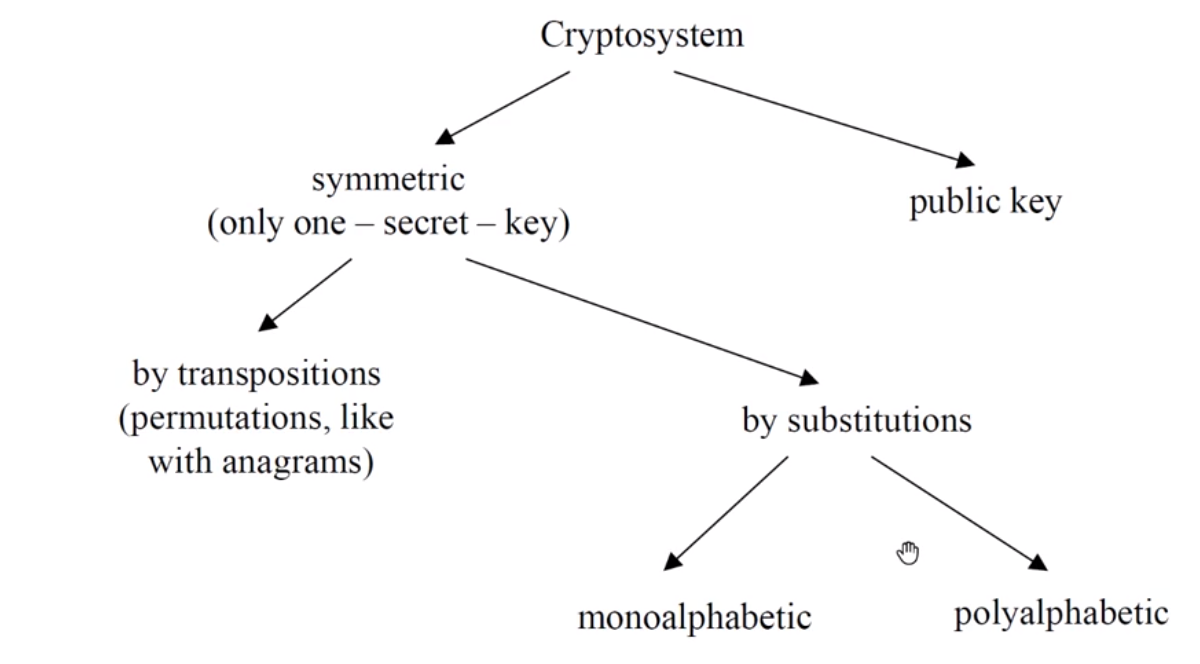
\includegraphics[width=\linewidth]{immagini/img31}
\end{figure}

\begin{itemize}
		\item Crittosistemi per sostituzione: ogni lettera di $c$ è sostituita con una lettera di $\Sigma$
		\begin{itemize}
			\item Monoalfabetici: è sostituita sempre con la stessa lettera
			\item Polialfabetici: la sostituzione cambia durante il processo di cifratura
		\end{itemize}
		\item Crittosistemi di trasposizioni: le chiavi sono:
		\begin{itemize}
			\item Troppo facili da trovare oppure
			\item Troppo difficili da ricordare
		\end{itemize}
	\end{itemize}

Possiamo usare un crittosistema polialfabetico da solo, oppure comporre trasposizione e sostituzione (product ciphers).

Per quanto un'informazione può rimanere segreta? Dipende da diversi fattori:
\begin{itemize}
	\item Chi è l'avversario: conoscenza matematica, potenza computazionale, budget, quanto guadagna a rompere...
	\item Avanzamento della tecnologia
	\item Dimostrazione di ipotesi matematiche non dimostrate oggi (es. oggi non è dimostrato problema fattorizzazione)
\end{itemize}

\newpage

\subsubsection*{Crittoanalisi dei crittosistemi monoalfabetici}
Ogni linguaggio naturale ha una distribizione di probabilità per le lettere che lo definisce, ad esempio in inglese:

\begin{figure}[h]
	\centering
	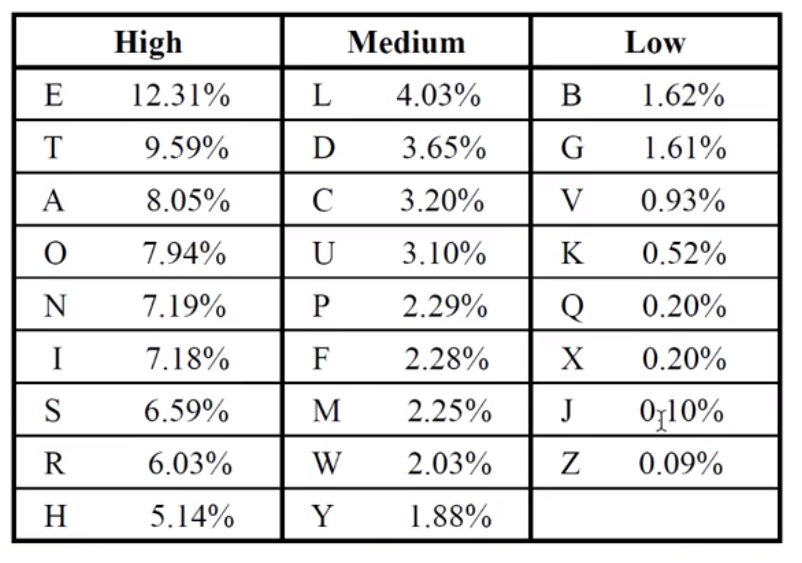
\includegraphics[width=0.65\linewidth]{immagini/img32}
\end{figure}

Una strategia per rompere un sistema monoalfabetico è contare la frequenza con cui compaiono le lettere, mettiamo ad esempio che in un testo cifrato la lettera \texttt{P} compaia 12 volte su 100: è molto probabile che essa sia una \texttt{E} o una \texttt{T} e così via (difficlmente, anzi impossibile sia una \texttt{Z}!).
Questo ovviamente nell'ipotesi di conoscere la lingua che sto cercando di decifrare.

Quindi la crittoanalisi di crittosistemi monoalfabetici si basa sull'analisi delle frequenze delle lettere. Questo ragionamento si basa sul fatto che la sostituzione delle lettere non cambia le frequenze.

Per difendersi da un attacco di questo tipo cosa si fa?
\begin{itemize}
	\item Lettere nulle: si aggiungono nel plaintext delle lettere a bassa frequenza, non fanno parte del messaggio
	\item Omofone: assumiamo di utilizzare $\Sigma=\{A,B, ...,Z\}$ e $\Gamma=\{0,1,2,...,99\}$ come alfabeti per \textit{PT} e \textit{CT}:
	\begin{itemize}
		\item Siccome la lettera \texttt{E} occorre il 12\% delle volte, associamo ad essa 12 simboli di $\Gamma$ (chiamati gli omofoni di \texttt{E})
		\item Quando cifriamo \texttt{E} si sceglie casualmente uno di questi simboli ($\rightarrow$ cifratura casuale)
		\item La scelta può essere anche fatta "a mano" in modo da appiattire le frequenze
	\end{itemize}
\end{itemize}

\subsubsection*{Crittoanalisi dei crittosistemi polialfabetici}
Le lettere in questo caso sono sempre sostituite in maniera diversa, ma se consideriamo vettori di lettere (coppie, triple, n-uple...), allora esse sono sostiutite sempre nello stesso modo.\\
Ad esempio nel crittosistema di Hill, la \texttt{H} in \texttt{HA} viene cifrata in modo diverso dalla \texttt{h} in \texttt{HE}, però queste due ultime coppie sono cifrate sempre nello stesso modo.
Quindi da un certo punto di vista diventa un monoalfabetico.
